\documentclass[sigconf]{acmart} 

\begin{comment}
\usepackage{booktabs} % For formal tables
\usepackage[T1]{fontenc}
\usepackage{graphicx}
\usepackage{tabularx}
\usepackage{textcomp}
\def\BibTeX{{\rm B\kern-.05em{\sc i\kern-.025em b}\kern-.08em
  T\kern-.1667em\lower.7ex\hbox{E}\kern-.125emX}}
\usepackage{booktabs} % For formal tables
\usepackage{cancel}
\usepackage{changes}
\usepackage{graphicx}
\end{comment}

\usepackage{colortbl} % Importa il pacchetto colortbl
\usepackage{xcolor,todonotes} 
\usepackage{url}
\usepackage{algorithm}
\usepackage{algorithmic}
\usepackage{amsmath}
\DeclareMathOperator*{\argmax}{\arg\!\max}
\usepackage{xspace}
\newcommand{\TransHI}{TransHySeCo\xspace}
\newcommand{\MostProbableClass}{mpc\xspace}
\newcommand{\counter}{\textsf{cnt}\xspace}
\definecolor{darkgreen}{RGB}{0,100,0}
\definecolor{lightgray}{gray}{0.9}
\newcommand{\elisa}[1]{{\color{darkgreen}#1}}
\newcommand{\nacera}[1]{{\color{violet}#1}}
\newcommand{\yue}[1]{{\color{blue}#1}}


%% \BibTeX command to typeset BibTeX logo in the docs
\AtBeginDocument{%
  \providecommand\BibTeX{{%
    Bib\TeX}}}

%% Rights management information.  This information is sent to you
%% when you complete the rights form.  These commands have SAMPLE
%% values in them; it is your responsibility as an author to replace
%% the commands and values with those provided to you when you
%% complete the rights form.
\setcopyright{acmlicensed}
\copyrightyear{2025}
\acmYear{2025}
\acmDOI{XXXXXXX.XXXXXXX}

%% These commands are for a PROCEEDINGS abstract or paper.
\acmConference[KRR]{KRR@40th ACM/SIGAPP Symposium On Applied Computing}{March 31 - April 4, 2025}{Sicily, Italy}
%%
%%  Uncomment \acmBooktitle if the title of the proceedings is different
%%  from ``Proceedings of ...''!
%%
%%\acmBooktitle{Woodstock '18: ACM Symposium on Neural Gaze Detection,
%%  June 03--05, 2018, Woodstock, NY}
\acmISBN{978-1-4503-XXXX-X/18/06}

\begin{document}
\title{A Hybrid Self-Correcting Approach for Embedding
Ontology-based Knowledge Graphs}
\titlenote{Produces the permission block, and
  copyright information}
%\subtitle{Extended Abstract}
%\subtitlenote{The full version of the author's guide is available as \texttt{acmart.pdf} document}
  
\renewcommand{\shorttitle}{SIG Proceedings Paper in LaTeX Format}

\begin{comment}
    
\author{Elisa Mariani}
\affiliation{%
  \institution{LISN, Paris-Saclay University }
  \city{Gif sur Yvette} 
  \country{France}
  \postcode{91190}  
}
\email{elisamariani1999@outlook.it}

\author{Nac\'era Seghouani}
\affiliation{%
  \institution{LISN, Paris-Saclay University }
  \city{Gif sur Yvette} 
  \country{France}
  \postcode{91190}  
}
\email{nacera.seghouani@lisn.fr}

\author{Yue Ma}
\affiliation{%
   \institution{LISN, Paris-Saclay University }
  \city{Gif sur Yvette} 
  \country{France}
  \postcode{91190}  }
\email{yue.ma@lisn.fr}
% The default list of authors is too long for headers}
\renewcommand{\shortauthors}{E. Mariani et al.}
\end{comment}

\begin{abstract}
One significant challenge in Knowledge Graph (KG) \textit{Embedding} is the generation of \textit{negative triples}. Negative triples are essential as they enable a training model to distinguish between relationships that exist within the KG and those that do not.
In this paper, we propose TransHySeCo approach: a Hybrid and Self-Correcting approach for embedding knowledge graphs. TransHySeCo is based on a hybrid training 
%to learn the KG embeddings
using both the domain semantics provided in the ontology related to the KG and the topology underlying the graph structure. Moreover, it is self-correcting. It generates new negative triples by leveraging the embeddings from previous training iterations and the \emph{(quasi-)true negatives} obtained with the \emph{ontology-based negative generation} method  proposed in this paper. 
%These new true negative triples are paired with the corresponding positive ones in a subsequent training step. 
The self-correction terminates when  no new \emph{(quasi-)true negative} triple  is generated. 
%We defined, implemented and evaluated 
%The whole framework includes   three main phases: pre-processing, training, and negative triples update, where the third phase is a prerequisite for the self-correct training. 
To evaluate TransHySeCo, we conducted  experiments on different benchmark datasets and assessed the embeddings' effectiveness for the link prediction task. %, by comparing  to TransE, TransR, TransOWL, and TransROWL approaches.
%state-of-the-art methods that inject background knowledge into KG embedding models. 
%The results position TransHySeCo as a promising solution for ontology-based knowledge graph embedding. 
The results show that TransHySeCo provides KG embeddings of promising  quality for link prediction.
\end{abstract}
% The code below should be generated by the tool at
% http://dl.acm.org/ccs.cfm
% Please copy and paste the code instead of the example below. 
% 

\begin{CCSXML}
<ccs2012>
   <concept>
       <concept_id>10010147.10010257.10010293.10010297.10010299</concept_id>
       <concept_desc>Computing methodologies~Machine learning approaches</concept_desc>
       <concept_significance>500</concept_significance>
       </concept>
   <concept>
       <concept_id>10003752.10003790.10003797</concept_id>
       <concept_desc>Theory of computation~Description logics</concept_desc>
       <concept_significance>500</concept_significance>
       </concept>
   <concept>
       <concept_id>10003752.10003790.10003794</concept_id>
       <concept_desc>Theory of computation~Automated reasoning</concept_desc>
       <concept_significance>500</concept_significance>
       </concept>
 </ccs2012>
\end{CCSXML}

\ccsdesc[500]{Computing methodologies~Machine learning approaches}
\ccsdesc[500]{Theory of computation~Description logics}
\ccsdesc[500]{Theory of computation~Automated reasoning}


\keywords{Knowledge Graph,  Ontology,  Translational Embedding, Link Prediction}

\maketitle

\section{Introduction}
The advent of Knowledge Graphs (KG) embeddings, transforming KG entities and relations into vector spaces, enhances KG utility for machine learning tasks 
\cite{reccommendationSystems,applications,NLP_applications,NLP_questionAnswering,NLP_sentimentAnalysis}, including  link prediction \cite{linkPred_with_embeddings,linkPred_with_embeddings2,linkPred_with_embeddings3} and triple classification \cite{tripleclass1,tripleclass2}. %\cite{GeAl2023}. 
These embeddings aim to minimize information loss, primarily utilizing positive and negative triples for training. Positive triples, drawn directly from the KG, represent true information, while negative triples, artificially generated, signify false or non-existent KG information \cite{neg1,neg2,neg3,neg4}. During training, embeddings learn to differentiate factual content from falsehoods. 
It is therefore pivotal to ensure that negative triples are genuinely incorrect and that positive triples are truthful and that they are not the result of a noisy or incomplete KG \cite{LR2023}.  A foundational translational embedding approach TransE, proposed by Bordes et al. \cite{bordes}, pairs each positive triple with a randomly generated negative during training. TransOWL, introduced by D’Amato et al.  \cite{transrowl}, as well as other numerous models in the literature \cite{NEURIPS2019_ontoEmbedding,WIHARJA2020100616,transrowl,paperiterative}, leverages the background knowledge contained within ontologies to craft negative samples, aiming for a more informed and beneficial generation process that supports the learning mechanism more effectively. Other approaches harness the intrinsic structure of the KGs. Among these, SANS approach,  adopted by Ahrabian et al. \cite{sanspaper} creates negative triples by substituting entities within a positive triple based on its neighborhood in the KG. 
 A different approach defined in \cite{paperiterative} applies first a link prediction algorithm with embeddings trained with a known algorithm, and then identifies incorrect predictions against an ontology, and uses these as negative feedback to refine the model through iterative training. 
Despite community research progress these approaches exhibit notable limitations:\\
    \noindent \textbf{(i)} Ontologies may not cover all entities and relationships, leading to unbalanced and unrepresentative training data.\\
    \textbf{(ii)} Structure-based approaches might overlook some semantic nuances that are captured in ontologies but absent in KGs. \\
    \textbf{(iii)} The presence of noise in KGs can compromise the integrity of positive triples, inadvertently training models on inaccuracies. Although the literature includes methods for fact validation and techniques for eliminating inconsistencies \cite{inconsistenciesinKG,topper,bonatti}, these are rarely incorporated into the embedding processes.\\
    \textbf{(iv)} The iterative method of \cite{paperiterative} restricts the number of negative triples available for self-correction, as the link prediction algorithm is not designed to identify incorrect triples, resulting in a potentially low count of such examples.

In this work, we present \TransHI, a novel, \textit{hybrid}, and \textit{self-correcting} approach to embed KGs, specifically aimed at enhancing link prediction efficacy. \TransHI aims to mitigate all the aforementioned problems related to the state of the art algorithms.
Our main contributions are:\\  
  \textbf{(1)} An efficient algorithm to remove inconsistencies and reduce noise within the positive triples of a KG (limitation \textbf{iii});\\
  \textbf{(2)} A method to create negative samples by blending semantics with graph topology, overcoming ontology limitations and semantic oversights (limitations \textbf{i}, \textbf{ii}); \\
  \textbf{(3)} A self-correct approach that, differently from \cite{paperiterative}, exploits a triple classification task, applied to a large number of \textit{(quasi-)true negative} triples, to spot misclassified true negatives, that are used as negative triples for the next self-correct training (limitation \textbf{iv}).\\
%\\
 % \textbf{(4)} The \TransHI framework has been evaluated on the link prediction task and its performances compared to the performances of models like TransE, TransOWL, TransR \cite{transR} and TransROWL \cite{transrowl} on different kind of benchmarks.
  
The paper is organised as follows. Section \ref{sect:overview} introduce an overview of \TransHI framework. 
%the main notations and present the principal phases of \TransHI framework. 
Sections \ref{sect:preprocessing}, \ref{sect:initialiteration}, \ref{sect:update} and \ref{sect:selfcorrect} detail the different phases of \TransHI. Section \ref{sect:evaluation}  presents   our evaluations showing that \TransHI  outperforms popular models like   TransOWL, TransR \cite{transR} and TransROWL \cite{transrowl} on various benchmarks. Section \ref{sect:relatedwork} discusses related work 
on KG embeddings. Section \ref{sect:conclusion} %discusses the results and their interpretation.  Section \ref{sect:future} 
concludes the paper with the perspectives of our approach.

\section{\TransHI Overview}
\label{sect:overview}
Let $\mathcal{O}$ be a domain ontology characterized by a set of terminological axioms   defined on a set of concepts $\mathcal{C}$ and a set of roles $\mathcal{R}$ in a given profile of OWL standard\footnote{https://www.w3.org/OWL/}. %\todo{$N_C, N_R, N_E$ may be better to distinguish from the embedding $\mathcal{E}$}
%(cf. Section \ref{sect:notations} for a formal  definition). 
The set $E$ denotes the set of entities. A knowledge graph $\mathcal{G}$ is a set of triples $(h,r,t)$, where $h\in E$, $r\in \mathcal{R}$, $t\in E$ if $r\not= type$ otherwise $t\in \mathcal{C}$, where  $type$ denotes the instance relation  as \textit{rdf:type} in RDF standard\footnote{\url{https://www.w3.org/TR/rdf11-concepts/}}.  


%learn a knowledge graph embedding $\mathcal{E}$ of $\mathcal{G}$ able to predict new triples (facts) based on existing positive and negative training triples, denoted below $S$ and $S'$, respectively.
%Let $\mathcal{O}$ be an ontology defined by a set of concepts and properties and let $\mathcal{A}$ the set of axioms that specifies the domain knowledge. 
%We assume a set of concept names $N_c$, a set of role names $N_r$ and a set of entity names $N_e$. The top and bottom concepts, denoted $\top$ and $\bot$ respectively, are two special concept names representing owl:Thing and owl:Nothing in OWL standard. And type is a special role, corresponding to rdf:type in RDF standard. A triple is $(e1,r,e2)$, where $e1,e2\in N_e, r\in N_c$. A knowledge graph (KG) is a set of triples that specifies the factual assertions. 
%An ontology is a set of axioms built from $N_c$, $N_r$ and $N_e$ by a set of logical connectors $op$(for example intersection, union, negation, value restriction) for an ontology language. Ontology axioms specify the domain knowledge. In this paper, we 
%The main challenging issues addressed in this paper are related to:
%(i) how to reduce the inconsistencies present in the knowledge graph to make positive triples relevant for the training? 
%(ii) how to generate true negative triples using the domain knowledge and, additionally, how to combine the graph topology knowledge with the semantics?
%(iii) how to make the training self-correct in order to improve the quality of the predictions? 
\begin{figure}[t]
\centering
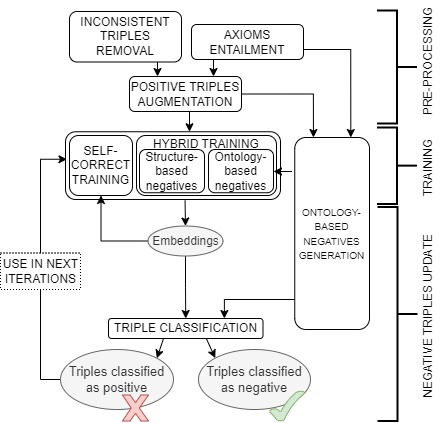
\includegraphics[width=0.5\textwidth]{Images/overview.jpg}
\caption{\TransHI approach Framework}
\label{fig:overview}
\end{figure}
%To tackle these issues we define 
%a Hybrid Self-correcting Approach for embedding knowledge graphs called \TransHI. 
%Figure \ref{fig:overview} depicts the overall \TransHI framework defined by the three following main phases:\\
The objective of  \TransHI is to define a knowledge graph embedding approach that mitigates the limitations presented above and outperforms in the link prediction task. We achieve this by leveraging the deep semantic information provided by the ontology associated to the KG, which is  key to the entire framework of  \TransHI, depicted in Figure \ref{fig:overview}, and includes three components:\\
\textbf{Pre-processing phase} aims to remove inconsistent triples from the KG  and to  enrich it by inferring new positive triples. This step requires effective inconsistency handling and inference methods.\\ 
     \textbf{Training phase} includes a hybrid training and a self-correct training. \TransHI develops a novel methods for generating negative samples based on ontology and KG.  Hybrid training is performed once over both structure-based negatives and ontology-based negatives. 
     %aims to learn the KG embedding with positive triples $\in S$ and negative triples $\in S'$, minimizing a loss function $L$. %(Section. \ref{sect:initialiteration}). 
    % The generation of negative triples    exploits initially both the KG structure and the domain ontology. 
     For   subsequent iterations, self-correct training is performed, where positive samples are paired with the negative samples discovered in the Negative Triples Update 
     phase below.\\
     \textbf{Negative Triples Update phase} prepares new negative triples to be used during the self-correct training by exploiting the embeddings created in the previous training and a triple classification task defined in \TransHI. Note that the triple classification is  purely based on automated ontology  reasoning without requiring additional labelled benchmark. 

  %More specifically, we define a linear algorithm to remove inconsistent triples wrt. $\mathcal{O}$ and $\mathcal{G}$. We also enrich the training subgraph using ontological entailment. This augmentation allows to generate new positive triples exploiting domain knowledge.
  %
  %contains the initial training iteration and the self-correction training. The difference of these two modes is the way we create the positive and negative samples. 
  %For the initial training, negative samples are generated from positive ones based on structure and ontology. 
  %

%The details of each phase are presented in Section \ref{sect:preprocessing}, \ref{sect:initialiteration}, \ref{sect:update} and \ref{sect:selfcorrect}.
%%%%%%%%%%%%%%%%%%%%%%%%%%%%%%%%%%%
%%%%%%%%%%%%%%%%%%%%%%%%%%%%%%%%%%%
%%%%%%%%%%%%%%%%%%%%%%%%%%%%%%%%%%%
%%%%%%%%%%%%%%%%%%%%%%%%%%%%%%%%%%%

\section{Pre-processing}
\label{sect:preprocessing}

The pre-processing    aims to first remove the triples that make $\mathcal{O} \text{ and } \mathcal{G}$ inconsistent, resulting in a sub-graph $\mathcal{G}_1 \subseteq \mathcal{G}$ such that $\mathcal{G}_1$ is consistent with $\mathcal{O}$. Then the positive triple augmentation  is achieved using $\mathcal{G}_1$ and $\mathcal{O}$   to generate new positive training triples. 


%Clearly, $O\cup G_1\cup T$ is consistent. 
%\todo[inline]{The triple augmentation step is performed only on the training triples, not on all G\_1}
 % \begin{itemize}
 %    \item Inconsistencies Removal: to identify and remove inconsistencies in the KG;
 %    \item Ontology Axioms Entailment: new axioms are entailed from the ones contained in the ontology;
 %    \item Positive Triples Augmentation: new positive triples are entailed from the KG and the ontology;
 %  \end{itemize}


%$(x, Equiv.Class, y)$, $(x,Disj.Class,,y)$, $(x,Disj.Prop,y)$, $(x, SubClass, z)$, $(x, SubProp, z)$, $(x, Domain, y)$,$(x, Range, y)$, $(a,InverseProp,b)$, $ (a,SameAs, b), $  $(a,type, Symmetric)$, $(a,type, Funct)$, $ (a,type, InvFunct)$, and $ (a,type, Transitive).$
%: $Equiv.Class,$ $Disj.Class, $ $SubClass,$ $SubProp, $ $Disj.Prop, $ $Disj.Class,$ $ Domain, Range,$ $ InverseProp,$ \ $Symmetric,$ $Funct,$ $Transitive, $ $ InvFunct, SameAs$.

\subsection{Basic Notations}\label{sect:notations}
Following the OWL standard\footnote{\url{https://www.w3.org/TR/owl2-primer/}}, 
the top and bottom concepts, denoted $\top$ and $\bot$ represent, \textit{resp.}, $owl$:$Thing$ and $owl$:$Nothing$. An ontology is a set of triples $(x,y,z)$, whose forms   are given below. 
% in the form: 
(i) $(x,r,y), r\in\{EquivClass, DisjClass, SubClass, SubProp,$ $DisjProp, DisjClass, Domain, Range, InverseProp\}$; or (ii) $(x,type, y), y\in\{Symmetric,$ $Funct,$ $Transitive, $ $ InvFunct\}$.
%the semantics of an OWL ontology and knowledge graph is defined by interpretations. 
The semantics of an OWL ontology $\mathcal{O}$ and knowledge graph $\mathcal{G}$ defined by interpretations. 
An interpretation 
$I=(\Delta^I, \cdot^I)$, where $\Delta^I\not=\emptyset$ is the domain of the interpretation and $\cdot^I$ is a mapping that maps concepts, roles, and entities is defined as follows: $\top^I=\Delta^I, \bot^I=\emptyset$, 
$C^I\subseteq \Delta^I$ for a concept $C$, $r^I\subseteq \Delta^I\times \Delta^I$ for a role $r\not= type$, and $e^I \in\Delta^I$. $I$ satisfies an ontology $\mathcal{O}$ if it satisfies each axiom $(x,y,z)\in \mathcal{O}$, denoted by $I\models (x,y,z)$.
%An interpretation $I=(\Delta^I, \cdot^I)$, where $\Delta^I$ is a non-empty domain and $\cdot^I$ maps concepts, roles, and entities, provides the semantics. $I$ satisfies an ontology $\mathcal{O}$ and a knowledge graph $\mathcal{G}$ if it adheres to specified conditions for each axiom and triple in $O$ and $\mathcal{G}$.
These axioms include equivalence, disjointness, subclass and subproperty relationships, domain and range specifications, inverse properties, and characteristics like symmetry, asymmetry, irreflexivity, functionality, transitivity, and inverse functionality. A knowledge graph
$\mathcal{G}$ is  consistent \textit{wrt.}  $\mathcal{O}$, if it exists $I$ that satisfies both  $\mathcal{G}$  and  $\mathcal{O}$, denoted by $I \models \mathcal{O}\cup\mathcal{G}$. A triple $(x,y,z)$ is entailed from  a knowledge graph $\mathcal{G}$  and an ontology $\mathcal{O}$, written $\mathcal{O}\cup\mathcal{G}\models (x,y,z)$, if for each interpretation $I$ satisfying  $\mathcal{O}$ and  $\mathcal{G}$, it also satisfies $(x,y,z)$. That is, $I\models (x,y,z)$  if $I\models \mathcal{O}\cup\mathcal{G}$.



%We first review some fundamental definitions following the OWL standard\footnote{\url{https://www.w3.org/TR/owl2-primer/}}. 
%The top and bottom concepts, denoted $\top$ and $\bot$ represent, resp., $owl$:$Thing$ and $owl$:$Nothing$. An ontology is a set of triples $(x,y,z)$, whose forms   are given below, along with the semantics of an OWL ontology and knowledge graph defined by interpretations. 
% in the form: (i) $(x,r,y), r\in\{EquivClass, DisjClass, SubClass, SubProp,$ $DisjProp, DisjClass, Domain, Range, InverseProp\}$; or (ii) $(x,type, y), y\in\{Symmetric,$ $Funct,$ $Transitive, $ $ InvFunct\}$.
%the semantics of an OWL ontology and knowledge graph is defined by interpretations. 
%An interpretation is 
%$I=(\Delta^I, \cdot^I)$, where $\Delta^I\not=\emptyset$ is the domain of the interpretation and $\cdot^I$ is a mapping that maps concepts, roles, and entities in the following manner: $\top^I=\Delta^I, \bot^I=\emptyset$, 
%$C^I\subseteq \Delta^I$ for a concept $C$, $r^I\subseteq \Delta^I\times \Delta^I$ for a role $r\not= type$, and $e^I \in\Delta^I$. An interpretation $I$ satisfies an ontology $O$ if it satisfies each axiom $(x,y,z)\in \mathcal{O}$, denoted by $I\models (x,y,z)$, as specified next:
%\begin{itemize}
  %\item $I\models(e, type, C)$ if $e^I\in C^I$.
%   \item $I\models(x, r, y)$, if it holds that $x^I= y^I$ for $r\in\{EquivClass,EquivProp\}$.
    %\item $I\models(x, EquivProp, y)$, if $x^I= y^I$.
%    \item $I\models(x, r, y)$, if $x^I\cap y^I=\emptyset$ for $r\in \{DisjClass$, $DisjProp\}$.
%    \item $I\models(x, r, y)$, if $x^I\subseteq y^I$ for $y\in \{subClass$, $subProp\}$. 
%    \item $I\models(r, Domain, x)$, if for any $(p,r,q)$, $p^I \in x^I$.
%    \item $I\models(r, Range, y)$, if for any $(p,r,q)$, $q^I \in y^I$.
%    \item $I\models (a,InverseProp,b)$, if $I\models (x,a,y) $ if and only if $I \models (y,b,x)$.
%    \item $I\models (a,type, Symmetric)$, if it holds that $I\models (x,a,y) $ if and only if $I \models (y,a,x)$.
 %   \item $I\models (a,type, Asymmetric)$, if it holds that $I\models (x,a,y) $ if and only if $I \not\models (y,a,x)$.
%    \item $I\models (a,type, Irreflexive)$, if it holds that %$I\models (x,a,y) $ if and only if
%    $I \not\models (x,a,x)$.
%    \item $I\models (a,type, Funct)$, if it holds that $I\models (x,a,y), I\models (x,a,z) $ imply that $y^I = z^I$.
%    \item $I\models (a,type, Transitive)$, if it holds that $I\models (x,a,y), I\models (y,a,z) $ imply that $I\models (x,a,z)$.
%    \item $I\models (a,type, InvFunct)$, if it holds that $I\models (x,a,y), I\models (z,a,y) $ imply that $x^I = z^I$.
   % \item $I\models (a,SameAs, b)$, if  $a^I = b^I$. 
%\end{itemize}
%An interpretation satisfies a knowledge graph $\mathcal{G}$ if it satisfies all the triples in $\mathcal{G}$ defined below:
%\begin{itemize}
%    \item $I\models(e, type, C)$, if $e^I\in C^I$.
%    \item $I\models(x, r, y)$, if $(x^I,y^I)\in r^I$.
%    \item $I\models(x, sameas, y)$, if $x^I=y^I\in \Delta^I$.
%\end{itemize}    


 
%To simplify notation, we use triples and the set of triples 
\subsection{Inconsistent Triples Removal}
%\begin{definition}[Inconsistent triples]
%A triple $t$ is an inconsistent triple wrt. $\mathcal{A}$ and  $\mathcal{G}$ if $ \mathcal{A}\cup \mathcal{G} \cup t $ is inconsistent. 
%\end{definition}
%\todo[inline]{I removed $\cup$ it's confusing notation with sets perhaps another operator. (The $\cup$ means exactly the set union of the set of ontology axioms and KB triples. For a better readability, I only use it in lemma/proposition.}
Given an ontology $\mathcal{O}$, it is known that if  $\mathcal{G}$ is inconsistent \textit{wrt.}  $\mathcal{O}$, there can be different subgraphs of $\mathcal{G}$ that are consistent with $\mathcal{O}$. It is known that the computation of all the maximal consistent subgraphs is a NP-hard problem even for tractable ontology languages, such as $OWL2EL$ \cite{PenaPhD}. In \TransHI, we explore a linear algorithm to get one particular consistent subgraph from $\mathcal{G}$ wrt. $\mathcal{O}$. 
For each entity $e \in E$, we define the set $T_e \subseteq \mathcal{G}$ as the set of triples where $e$ appears. 
We denote $\counter(e,c)$ the counter of $e$ \textit{wrt.} a concept $c\in \mathcal{C}\setminus\{\top\}$ as the number of triples in $T_e$
that can infer that $e$ is of type $c$ \textit{wrt.}  $\mathcal{O}$:
$ \counter(e,c)=
  \#\{t \in T_e \mid \mathcal{O} \cup \{t\} \models (e,type,c)\}$
Intuitively, $\counter(e,c)$ is a metric to measure the times of an entity $e$ being an instance of the class $c$ under ontology entailment.
%\smallskip

\begin{small}
\begin{example}\label{exam:cnt}
\noindent Consider  $\mathcal{G}$ and  $\mathcal{O}$ defined as:
\begin{scriptsize}
    \begin{align*}
    \mathcal{G}=&\{(Amsterdam, type, Agent), (Amsterdam, timezone, EuropeanTime),\\
    &(BaruchSpinoza, birthplace, Amsterdam), (DutchRepublic, capital, Amsterdam)\},\\
    \mathcal{O}=&\{(capital, Range, City),(City, subClass, Location),\\
    &(capital, Domain, Country), (Location, EquivClass, Place),\\
    &(timezone, Domain, Location), (birthplace, Range, Place)\}.
    \end{align*}
\end{scriptsize}
$\counter(Amsterdam, Place)=3$ because $(Amsterdam, type, Place)$ can be inferred from $\mathcal{O}$ with triples 2, 3, and 4 in $\mathcal{G}$. However, $\counter(Amsterdam, Agent)=1$ as $(Amsterdam, type, \\ Agent)$ is directly from the first triple in $\mathcal{G}$.
\end{example}
\end{small}

\noindent Let $\MostProbableClass(e)$ be one of the most probable concepts, the concepts with the largest counters for $e$: \(\MostProbableClass(e) \in \argmax_{c\in \mathcal{C},\ \counter(e,c)>0} \counter(e,c)\). Let $T_{\MostProbableClass}$ be the set of triples where each $e$ is associated to its most probable class: \\$T_{\MostProbableClass}=\{ (e,type,\MostProbableClass(e))\mid \counter(e,c)\not=0 \}$. %If there is such one, we have that $T_{\MostProbableClass}$ consistent with $\mathcal{O}$. 

\begin{small}
\begin{example}[Example \ref{exam:cnt} contd.] \label{exam:2}
$\MostProbableClass(Amsterdam)= Place,\text{ and } T_{\MostProbableClass}=\{(Amsterdam,\\ type, Place)$, $(DutchRepublic, type, Country)\}$. Note that no type information can be entailed for $BaruchSpinoza$  so it is missing in $T_{\MostProbableClass}$. 
\end{example}
\end{small}

\noindent In this example, $T_{\MostProbableClass}$ is consistent with $\mathcal{O}$. Indeed, this is a general conclusion as shown by the following lemma.

\begin{lemma}\label{lemma:consis}
  $\mathcal{O}\cup T_{\MostProbableClass}$ is consistent.
\end{lemma}
% \begin{proof} 
% Since $\mathcal{O}$ is consistent, we assume $\mathcal{I}$ is an interpretation satisfying $\mathcal{O}$. We extend $\mathcal{I}$ by defining $e^\mathcal{I} \in (\MostProbableClass(e))^I$, obtaining an interpretation denoted $\mathcal{I}'$. Clearly $\mathcal{I}'$ satisfies $\mathcal{O}$ and $T_{\MostProbableClass}$. So $\mathcal{O} \cup T_{\MostProbableClass}$ is consistent.
% \end{proof}
%\todo{to be proved or we don't put it as a lemma. }
%\begin{scriptsize}
%\begin{algorithm}[t]
%\caption{Inconsistent Triples Removal}
%\label{binarySearch pseudo}
%\begin{small}
%\textbf{binarySearch}$(subSetG,\mathcal{O},T)$
%\begin{algorithmic}[1]
%    \IF{\textit{isConsistent}($subSetG,\mathcal{O},T$)}
%            \STATE $T \gets T \cup subSetG$
%        \ELSE
%            \STATE $size\gets size(subSetG)$
%            \IF{$size > 1$}
%                \STATE Split $subSetG$ in half:$leftHalf$ and $rightHalf$
%                \STATE \textit{binarySearch}($leftHalf, \mathcal{O},T$)
%                \STATE \textit{binarySearch}($rightHalf, \mathcal{O}, T$)
  %          \ELSE
  %              \STATE The triple is inconsistent, remove it from KG. 
%            \ENDIF
%        \ENDIF 
%    \STATE Return $T$

%    \end{algorithmic}
%    \end{small}
%    \end{algorithm}
%    \end{scriptsize}


We defined a recursive $binarySearch$ procedure to remove the inconsistent triples with $\mathcal{O}$ from the original graph $\mathcal{G}$, starting with the consistent triple set $T \gets T_{\MostProbableClass}$ and 
$subSetG \gets \mathcal{G}$ as the set of triples to be checked for inconsistency with both $\mathcal{O}$ and $T$.  Each time, $binarySearch$ involves checking the consistency of  $subSetG \text{ and } \mathcal{O} \text{ and } T$. When consistent, the triples in $subSetG$ are added to $T$. Otherwise, $subSetG$ is divided into two halves, on each of which a recursive call of the $binarySearch$ algorithm is launched. 
If $|subSetKG|$ reaches one triple and the triple is still inconsistent, it is not added to $T$. After inconsistent triples removal the output is a new graph.

\begin{proposition}\label{prop:inconsistencyremoval}Let 
  $\mathcal{G}_1= binarySearch(\mathcal{G},\mathcal{O},T_{mpc})$. Then $\mathcal{G}_1 \cup \mathcal{O}$ is consistent.
\end{proposition}

% \begin{proof} By Lemma \ref{lemma:consis}, the $T_{mpc}$ is consistent with $\mathcal{O}$. By definition, $\mathcal{G}_1$ is obtained by calling Algorithm \ref{binarySearch pseudo} with an initial consistent set of triples $T_{mpc}$. In each subsequent binary search, as specified in Line 2, the triple set $T$ is merely increased with the triples that consistent with $O$ and the existing triples. So when the whole binary search procedure terminates, only a set of triples consistent with $\mathcal{O}$ is returned, that is, $\mathcal{G}_1 \cup \mathcal{O}$ is consistent.
% \end{proof}

\noindent In the subsequent phases of our framework, only the consistent triples $\mathcal{G}_1$ are considered.
The algorithmic complexity of this procedure applied to a graph $\mathcal{G}$ with $n$ triples is $O(nf(n))$, where $f(n)$ is the complexity of consistency checking on $n$ triples, which is polynomial for OWL2EL, OWL2QL and OWL2RL profiles of OWL2. This is significantly more efficient than the $O(2^n)$ complexity required to verify the consistency of all possible subsets of $n$ triples.
% In the subsequent pipeline steps, only consistent triples of the KG, denoted as $G_1$, are considered.

\subsection{Positive Triples Augmentation}\label{sect:triple-augmentation} 
Several studies have demonstrated the effectiveness of enriching KGs by applying ontology-based inference \cite{positiveTripleAugmentationSource1}\cite{positiveTripleAugmentationSource2}\cite{positiveTripleAugmentationSource3}.  In our approach, \TransHI, we exploit the inference by selecting  carefully the set of inference rules to generate new triples that are added to  $\mathcal{G}_1$. For instance,
\begin{small}
$(e,type,c), (c,SubClass,c') \models (e,type,c');$
\end{small} and 
\begin{small}
$(e_1,a,e_2), (a,EquivProp,b) \models (e_1,b,e_2);$
\end{small}
we thus derive from $\mathcal{G}_1$ a consistent set of positive training triples  $S$ which remains unchanged through all training phases of \TransHI, including the initial training and subsequent self-correction iterations.
We will further discuss the hybrid method for constructing negative triples for the initial training in Section \ref{sect:initialiteration} and outline the strategy for updating negative triples in Section \ref{sect:update}.



%%%%%%%%%%%%%%%%%%%%%%%%%%%%%%%%%%%
%%%%%%%%%%%%%%%%%%%%%%%%%%%%%%%%%%%
%%%%%%%%%%%%%%%%%%%%%%%%%%%%%%%%%%%
%%%%%%%%%%%%%%%%%%%%%%%%%%%%%%%%%%%

\section{Hybrid Training}
\label{sect:initialiteration}
%In the training of KG embedding models, each positive triple is matched with a negative one to ensure balanced learning based on the relationships present and absent in the knowledge graph. 
In \TransHI, each positive triple is matched with a negative one generated using a hybrid approach that combines ontology-based and structure-based methods, alongside a portion of randomly generated negatives. This allows a uniform training and improves generalization. The set of negative training triples is defined as follows: $$S'=S'_{Ont} \cup S'_{Str} \cup S'_{Rnd}.$$ 

For the training phase, essentially, any embedding model using positive and negative triple set, $S$ and $S'$, is suitable for our needs. Here, 
for simplicity of presentation, we use the simple but efficient TransE \cite{bordes} model, for which the general loss function %based on TransE embedding \cite{bordes} 
to be optimized using stochastic gradient descent (SGD) \cite{SGD}, is defined as:
$
%\begin{split}
L = \sum_{(h,r,t) \in S} \sum_{(h',r,t') \in S'} \min(0, \gamma +
f(e_h, e_r, e_t) - f(e_{h'}, e_r, e_{t'})),
%\end{split}
$
where $e_h, e_r \text { and } e_t$ are  the vector embeddings of $h, r \text { and } t$, respectively. We say the negative triple $(h',r,t')$ as ``paired" with the positive one $(h,r,t)$.
%It is important to note that we choose TransE as a baseline because it is basic and efficient. 
%\TransHI can be easily adapted to support any embedding model, and, with an increased number of self-correction training, it gives a way to yield better embeddings for link prediction. %, with which higher link prediction accuracy w.r.t. standard metrics is achieved. 
\noindent Then the loss function of \TransHI can be   expressed using the three kind of negative  triples as follows:
%\begin{small}
%\begin{scriptsize}
\[ 
\begin{split}
L= \sum_{(h,r,t) \in S_{Rnd}} \sum_{(h',r,t') \in S'_{Rnd}}  \max(0, \gamma + f(e_h, e_r, e_t) - f(e_{h'}, e_r, e_{t'})) \\
 + \sum_{(h,r,t) \in S_{Ont}} \sum_{(h',r,t') \in S'_{\text{Ont}}} \max(0, \gamma + f(e_h, e_r, e_t) - f(e_{h'}, e_r, e_{t'})) \\
 + \sum_{(h,r,t) \in S_{Str}} \sum_{(h',r,t') \in S'_{Str}} \max(0, \gamma + f(e_h, e_r, e_t) - f(e_{h'}, e_r, e_{t'})) 
\end{split}
\]     
%\end{scriptsize}
%\end{small}

\noindent Additionally, during the training of \TransHI, we ensure that \(S\cap S'=\emptyset\) and control the random component $S'_{Rnd}$ by a hyperparameter that is  optimized  empirically. 

In the  next sections, we define how ontology-based and structure-based triples, $S'_{Ont}$ and $S'_{Str}$, are generated.

\subsection{Ontology-based negative triples generation}
\label{sect:ontology-negative}

Given a positive triple $s\in S$, we create a negative-based triple $s'\in S'_{Ont}$ that is (highly possibly) inconsistent with $s$ leveraging ontological axioms: we call such negatives \emph{(quasi-)true negatives}.
%:
%$\{s\}\cup\mathcal{O}\models \neg s'.$
%This ensures that the generated triple is (almost) genuinely negative. 
%We call such a negative triple  \emph{(quasi-)true negatives} defined below: 
\begin{definition}
     A triple $s'$ is called \emph{true negative} wrt.  $S$ and  $\mathcal{O}$, if there is a triple $s\in S$ such that $\{s\}\cup\mathcal{O}\models \neg s'$.
\end{definition} 

In contrast to true negatives, quasi-true negatives take the assumption that sibling classes (classes that are at the same hierarchical level but represent different, distinct entities) are mutually disjoint to create inconsistency,  which is good practice, for instance for Biological and Biomedical Ontologies community \cite{bioinformatics/btt491}. 
\begin{definition}
  A triple $s'$ is called \emph{quasi-true negative} wrt.  $S$ and $\mathcal{O}$, if there is a triple $s\in S$ such that $\{s\}\cup\textsc{SiblingDisj}(\mathcal{O})\models \neg s'$, where $\textsc{SiblingDisj}(\mathcal{O}) $ is the ontology $\mathcal{O}$ enriched by adding disjoints among all sibling concepts.
\end{definition}

Given a positive triple $(h,r,t)\in S$, the different categories of negative triples in $S'_{Ont}$ are generated from ontological axioms as follows:\\
%are indicated in the following list:\\
\begin{small}
\noindent \textbf{O1)} $(h',r,t) \mbox{ if } r=type,
$ $(h', type,c)\in S$,  $ (t,DisjClass,c)\in \mathcal{O}$;\\
\textbf{O2)} $(h,r,d)\mbox{ if } r=type, 
(t,DisjClass,d)\in \mathcal{O}$;\\
\textbf{O3)} $(h,p,t)\mbox{ if } r\neq type, (r,DisjProp,p)\in \mathcal{O}$;\\
\textbf{O4)} $(h,r,h)\mbox{ if } r\neq type, (r,type,Irreflexive)\in \mathcal{O}$;\\
\textbf{O5)} $(t,r,h)\mbox{ if } r\neq type, (r,type,Asymmetric)\in \mathcal{O}$;\\
%\textbf{O6)} $(h',r,t)\mbox{ if } r\neq type$, there is no $c$ such that $(r,Domain,c)\in\mathcal{O}$ and $(h',type,c)\in S$;\\
\textbf{O6)} $(h',r,t)\mbox{ if }  r\neq type$, $(h',type,c)\in S$ but there is no $c$ such that   $(r,Domain,c)$;\\
%\textbf{O7)} $(h,r,t')\mbox{ if } r\neq type,(\nexists C|(r,Range,c)\in\mathcal{O},(t',type,c)\in S.)$\\
\textbf{O7)} $(h,r,t')\mbox{ if }  r\neq type$, $(t',type,c)\in S$ but there is no $c$ such that   $(r,Range,c)$.
%\yue{\textbf{O7)} $(h,r,t')\mbox{ if } (r,Range,c)\in\mathcal{O}, (c,DisjClass,d)\in\mathcal{O},$ and $ (t',type,d)\in S.$}
\end{small}
%\todo[inline]{I would say true (06-07)  and quasi-true negatives (O6'-O7'). }

%In the list, $E(C)$ refers to entities of the concept $C$ and $\mathcal{C}(x)$ to the concepts of entity $x$. 
Note that $\mathcal{O}$ and $S$ are enriched in Section \ref{sect:triple-augmentation}, then we have that  such created negatives are true or quasi-true negatives: 
    negative triples of  type O1-O5 are true negatives, and those of  type O6-O7 are quasi-true negatives.

%\begin{example}We consider a positive triple $(Tom Cruise,type, Actor)$ and  two ontological  axioms:
%$(Actor,DisjClass,Building), (Actor, DisjClass, Island)$. Following   O1 above, one can corrupt the %head of the positive triple by substituting it with entities belonging to concepts that are disjoint %from $Actor$, such as $Building$ or $Island$. 
%\end{example}
\begin{small}
\begin{example}
    Consider the positive triple $(Germany, capital, Berlin)\in S$ and an axiom $(capital, Domain, country)\in\mathcal{O}$. \\ If $(LesMiserable, type, book)\in S$, we can have an quasi-true negative triple $s'=(LesMiserable, capital, Berlin)$ by O6. $s'$ is highly possible to be a negative triple, though it does not cause inconsistency with $\mathcal{O}$.
\end{example}
\end{small}
%During training, when the initial positive triple is of the form (h, type, t),  negative triples of type O1 or O2 will be generated. Otherwise, negatives of type O3-O7 will be generated, with a preference for O3-O5 due to their typically lower number compared to O6 to O7. Indeed, 
$S'_{Ont}$ diverges from the set of negatives generated in TransOWL \cite{transrowl} due to the utilization of a broader range of axiom types, in greater quantity, facilitated by  ``Axioms Entailment", as defined in Section \ref{sect:triple-augmentation}. 

For the negatives related to Domain axiom (type O6), we have an intuitive true negative $(h',r,t)$  if $(r,Domain,c)\in\mathcal{O},$ $ (c,DisjClass,d)$ $\in \mathcal{O}$, and $(h',type,d)\in S$. However, this manner limits the number of generated negatives since it depends on the DisjClass axioms in $\mathcal{O}$.  O6 relaxes this requirement and introduces quasi-true negatives. The same reasoning is applied to the negatives of type O7. Such a large number of quasi-true negatives is essential for self-correct training in \TransHI. Types O1, O6, and O7 exclude entities not part of any concept, leading to potential training set imbalances. This is addressed by supplementing ontology-based triples with structure-based ones, proportionally to entities without concept instances, mitigating the issues `1' and `2' presented in section \ref{introduction}: balancing the ontological information but still capturing semantic nuances within it.

%For the negatives related to Domain axiom (type O6), we have an intuitive true negative $(h',r,t)$  if 
%the negatives should be built as: $(h',r,t)$ if %$ \exists c\in DomainClasses(r) $ and $ \exists c'\in Classes(h') $ and $ (c,DisjClass,c')\in \mathcal{O}$ 
%$(r,Domain,c)\in\mathcal{O},$ $ (c,DisjClass,d)\in\mathcal{O}$, and $(h',type,d)\in S$. However,
%This condition ensures that $(h',r,t)$ is inconsistent, but 
%this manner limits the number of generated negatives since it depends on the DisjClass axioms in $\mathcal{O}$.  O6 relaxes this requirement and introduces quasi-true negatives.  %have decided to relax this condition.  
%The same reasoning is applied to the negatives of type O7. Such a large number of quasi-true negatives is essential for self-correct training in \TransHI.

%The types of negatives O1, O6, O7 can not include entities that are not instances of any concept. This could lead to an unbalanced training set with underrepresented entities and uneven learning.  
%\todo{need highlight it? Elisa's answer: I would mention it because it is the reason for using a quantity of S'\_ont proportional to the number of entities that are not instancces of any concept}
%$S'_{Ont}$ may also be generatable for only part of $S$ because $O$ may lack information pertaining certain entities or relationships.
%These two issues are addressed by using structure-based triples not only when no ontology-based triples can be generated for the considered positive triple but also when they are generatable, in a quantity proportional to the number of entities that are not instances of any concept.

\subsection{Structure-based negative triples generation: $S'_{Str}$}

In \TransHI, the creation of structure-based triples  aligns with the principle employed in SANS\cite{sanspaper}. \TransHI enhances SANS by ordering the entities' neighbors: the $k$-hop neighbors of the entities to corrupt in order to form the negative triples are arranged in ascending order according to their Clustering Coefficient  (CC) \cite{CC1988}. We define $N_{cc}(x)$ the list of the $k$-hop neighbors of  $x$ in  the increasing order based on CC. Given $s\in S$, we create $s' \in S'_{Str}$ by substituting the head $h$ (or the tail $t$)  of $s$ with its $k$-hop neighbor with the lowest CC. This idea, inspired by Kaoudi et al. \cite{volkr}, prioritizes the use of entities in sparse regions of the graph. It's worth noting that,  each neighbor related to an entity is used only once in substution of such entity to create a negative triple. Theoretically, for two triples $(h1, r1, t1)$ and $(h2, r2, t1)$, $t1$ could be replaced by the same neighbor e.g., $t*$, resulting in two distinct negative triples $(h1, r1, t*)$ and $(h2, r2, t*)$. However,  our empirical observations revealed that reusing neighbors multiple times led to an excessive utilization of certain entities and the neglect of others during the learning process. 

\section{Negative Triples Update}
\label{sect:update}

We define the embedding of an entity $x$ produced during the previous training step as $e_x$. This phase aims to create  a set of new effective negative triples, $S'_{Corr}$, to be used during the following iteration of training.
To create such negative triples, at first a set $I$ of triples inconsistent with $S\cup \mathcal{O}$ is created. The triples in $I$ are then classified through a triple classification task and the misclassified triples constitute the set $S'_{Corr}$.
The presence of misclassified negative triples suggests room for improvement in their corresponding embeddings: using $S'_{Corr}$ as negative triples in a new training step we are able to ``correct" them. \\

%This approach is inspired by Jain et al.\cite{paperiterative}, where the embeddings not learned properly were identified through a link prediction task.

\noindent \textbf{Ontology-based Negatives ($I$) Generation.} Let $I$ be a set of quasi-true negative triples created following the ontology-based negatives procedure (Section \ref{sect:ontology-negative}). These are the candidates for use as negative triples in the subsequent self-correction training. Note that $I$ is different from the one used in the hybrid training phase. And a different negative triple set $I$ should be generated anew in each self-correction training to enhance the embedding. Furthermore, $|I|=Epochs \times |S|$ (where $Epochs$ are the number of training epochs used during training) to ensure that each epoch uses a distinct negative triple for a given positive triple $s$. \\

\noindent \textbf{Triple classification.} The triples in $I$ are classified as positive or negative using the generated embeddings. For each $(h,r,t)\in I$, \(f(e_h,e_r,e_t) = \lVert e_h + e_r - e_t \rVert_2^2\). If $f(e_h,e_r,e_t)<\delta(r)$, then $ (h,r,t)$ is classified as positive. Otherwise, it is  negative. $\delta(r)$ is defined as:\(\delta(r) = \max \{ f(e_h,e_r,e_t) \, | \, (h,r,t) \in S  \}.\)  %Utilizing distinct thresholds for each relation accounts for variations in scores between triples with different relations, accommodating the diversity of information in the embeddings. 
We define the set of  triples for self-correction as those misclassified according to the current embedding: \(S'_{Corr}=\{(h,r,t)\in I\mid f(e_h,e_r,e_t)<\delta(r)\}\) because the triples from $ I$ should all be classified as negative.

%Given the training epoch  $Epochs$, the number of such negative triples  for each positive $s\in S$ satisfies:  $$|\{s'\in I\mid s' \mbox{ is a (quasi-) true negative for }s\}|\leq Epochs.$$
% $\forall s \in S$:
% \[
% | \{ s' \in I \, | \, (s \text{ and } \mathcal{O}) \models \neg s' \} | \leq Epochs
% \] 
%where $Epochs$ are the training epochs used during the following training. 
%\todo{why on average?}Each $s \in S$ is used, on average, once per training epoch (Alg. \ref{2iter pseudo}). In the worst-case scenario, $|I|=Epochs*|S|$ is the maximum size of $|I|$ to be able to use all the triples within it. 

%Among all the triples, only those misclassified as positive by the current embedding, as detailed in the next section, can be used as negative triple in the next iteration of self-correction.
%In an extreme case, all negative triples are mis-classified, 
%Moreover, it is important to note that the triples from $I$ are not repeated in the new sets $I$ that will be generated in subsequent iterations.

%\todo[inline]{formalise it}
%\subsection{Triple Classification} The triples in $I$ are classified as positive or negative using the generated embeddings. For each $(h,r,t)\in I$,
%         \[f(e_h,e_r,e_t) = \lVert e_h + e_r - e_t \rVert_2^2\ .\]
%If $f(e_h,e_r,e_t)<\delta(r)$, then $ (h,r,t)$ is classified as positive. Otherwise, it is  negative. $\delta(r)$ is defined as:
%\[
%\delta(r) = \max \{ f(e_h,e_r,e_t) \, | \, (h,r,t) \in S  \}.
%\]
%Utilizing distinct thresholds for each relation accounts for variations in scores between triples with different relations, accommodating the diversity of information in the embeddings.
%We define the set of  triples for self-correction as those misclassified according to the current embedding:
%\[S'_{Corr}=\{(h,r,t)\in I\mid f(e_h,e_r,e_t)<\delta(r)\}\]
%because the triples from $ I$ should all be classified as negative.


\section{Self-correct Training}
\label{sect:selfcorrect}
The primary objective of the training iterations subsequent to the initial one is self-correction, leveraging the misclassified triples generated in the preceding iteration. 
The Algorithm \ref{2iter pseudo} outlines the functioning of self-correction in the iterations following the first.
The positive triples $S$, the score function $f$ and the embedding optimization via SGD remain the same with the first iteration. However, the negative triples $S'$, to avoid overfitting, are different:
\(S'= S'_{Corr} \cup S'_{RndC},\). $S'_{RndC}$ comprises negatives generated randomly under the following two empirical constraints, whose aim is to reduce the likelihood of generating false negatives and to avoid degrading the quality of the embeddings. For a   positive $s=(h,r,t)\in S$ and a randomly generated negative $(h',r',t')\in S'_{RndC}$ if and only if it satisfies:\\
\textbf{C1} (Line 10): \(f(e_{h'},e_{r'},e_{t'})>f(e_h,e_r,e_t)\) \\
\textbf{C2}  (Line 10,12): \((cos\_sim(e_h,e_{h'})<0\) and \(t'=t)\) or \\\( (cos\_sim(e_t,e_{t'})<0\) and \(h'=h)\)  


%where  $S'_{Corr}$ negatives aim to correct the embeddings of the misclassified triples (Line 9 of Alg. \ref{2iter pseudo}). Instead, $S'_{RndC}$ comprises negatives generated randomly under the following two empirical constraints, whose aim is to reduce the likelihood of generating false negatives and to avoid degrading the quality of the embeddings. 

%For a   positive $s=(h,r,t)\in S$ and a randomly generated negative  $(h',r',t')$ from $s$, $(h',r',t')\in S'_{RndC}$ if and only if it satisfies:

%$C1$ and $C2$ are defined as:
% \begin{itemize}
%     \item 
% \(C1: (h',r',t')\in S'_{RndC}\implies f(h',r',t')>f(h,r,t)\)
%     \item \(C2: (h',r',t')\in S'_{RndC}\implies(cos\_sim(e_h,e_{h'})<0\land t'=t)||(cos\_sim(e_t,e_{t'})<0\land h'=h)\),
% \end{itemize}
% %\(C2: (h',r',t')\in S'_{RndC}\implies(cos\_sim(e_h,e_{h'})<0\land t'=t)||\\ (cos\_sim(e_t,e_{t'})<0\land h'=h)\)\\
\noindent where $cos\_sim(e_x,e_y)$ is the cosine similarity function between the two embedding vectors. The first constraint is based on the definition of $f$, suggesting that $(h',r',t')$ is less likely to be  true than $(h,r,t)$. The second is based on the intuition that, to create a likely negative triple, the entity to be corrupted should be replaced with an entity that is substantially different from it. Substituting it with a similar entity might result in false negatives. Hence, it is preferred that the cosine similarity is low. The threshold for accepted similarity was determined empirically and set to 0. 
%Setting a lower threshold would further restrict the similarity between entities, which can be beneficial but also limits the pool of selectable entities. This could lead to overfitting on these entities, so it is better to keep the range of selectable entities as wide as possible. However, allowing a cosine similarity greater than 0 is risky as it implies some level of similarity between the two entities. %Both constraint 1 and 2 aim to reduce the likelihood of generating false negatives with the random approach, to avoid degrading the quality of the embeddings.

Given the two types of negatives,  the loss function becomes:
\begin{scriptsize}
\[
\begin{split}
L = \sum_{(h,r,t) \in S_{\text{Corr}}} \sum_{(h',r',t') \in S'_{\text{Corr}}} \max(0, \gamma + f(e_h, e_r, e_t) - f(e_{h'}, e_{r'}, e_{t'})) \\
 + \sum_{(h,r,t) \in S_{RndC}} \sum_{(h',r,t') \in S'_{RndC}} \max(0, \gamma + f(e_h, e_r, e_t) - f(e_{h'}, e_r, e_{t'})) 
\end{split}
\]
\end{scriptsize}

\noindent It is important to note that the negatives in $S'_{Corr}$ are created as the ontology-based negatives from their corresponding positive triples $S_{Corr}$.
Therefore the same consideration as in the hybrid training on entities without an associated class holds: therefore, negatives in $S'_{Corr}$ are used in a quantity inversely proportional to the percentage of entities that are not instances of any class (\(pct\_no\_class\_entities\), Line 5). Excessive use of $S'_{RndC}$ negatives can lead to overfitting, as entities with similarity $<0$ to a given one ($C2$) are limited. To address this, the percentage of triples subject to $C2$ is inversely proportional to the percentage of entities that are not instances of any class (Line 12). 
 %Given that the focus of this step is the self-correction, the training stops if $|S'_{Corr}|=0$.

\begin{algorithm}[t]
\caption{TransHySeCo self-correct training}
\begin{scriptsize}
\textbf{TransHySeCo\_Self\_Corr}(prev\_embeddings,$S'_{Corr}$,S)\\[-9pt]
    \begin{algorithmic}[1]
        \STATE Initialize embeddings with \textit{prev\_embeddings}
        \FOR{$i = 1$ \TO \textit{Epochs}, if {$|S'_{Corr}|$  $\neq$ 0}}
            \FOR{$j = 1$ \TO  $|S|$}
                \STATE Sample positive triple \((h, r, t)\) $\in$ S
                \IF{$\exists$ \(m\) $\in$ $S'_{Corr}$ paired to \((h,r,t)\) \AND rand\_num(0,100)$>$ \(pct\_no\_class\_entities\)}
                    \STATE Neg. triple \((h', r, t') \leftarrow m\)
                    \STATE Remove \(m\) from $S'_{Corr}$ 
                \ELSE
                    \IF{rand\_num(0,100)$>$\(pct\_no\_class\_entities\)}
                    \STATE Neg. triple \((h', r, t')\) $\leftarrow$ \textit{randomNegative}(h, r, t) satisfying  C1 \AND C2
                    \ELSE
                        \STATE Neg. triple \((h', r, t')\) $\leftarrow$ \textit{randomNegative}(h, r, t) satisfying C2
                    \ENDIF
                \ENDIF
                                    \STATE 
                \textit{updateEmbeddings}(h, r, t, h', r, t')
            \ENDFOR
        \ENDFOR
    \end{algorithmic}
    \label{2iter pseudo}
\end{scriptsize}
\end{algorithm}

\noindent\textbf{Continuation of the pipeline}.
The pipeline proceeds with an iterative succession of phases ``Negative Triples Update" and ``Training Self-correction".
The two termination conditions for the pipeline are: $I = \emptyset$, the absence of new ontology-based negatives generatable to conduct the classification task; $S'_{Corr} = \emptyset$, the absence of misclassified triples during the triple classification.

After completing  the\TransHI iterations, one can compare the quality of the embeddings obtained across various iterations and choose to use those of the highest quality for the preferred application context.

%%%%%%%%%%%%%%%%%%%%%%%%%%%%%%
%%%%%%%%%%%%%%%%%%%%%%%%%%%%%%
%%%%%%%%%%%%%%%%%%%%%%%%%%%%%%

\section{Experience and Evaluation}
\label{sect:evaluation}
%In each iteration of the hybrid and self-correction pipeline, novel embeddings are generated. The ultimate objective is to select the most optimal embeddings from one of these iterations. 
In this section, we present the experiments we conducted to evaluate \TransHI for link prediction purposes on three distinct real-world KGs:  DBPEDIA15k\cite{dbpedia}, YAGO\cite{YAGO}, and NELL\cite{nell}. 
The questions we aim to address are:\\
\textbf{(1)} To what extent is link prediction influenced by the use of \TransHI's pre-processing method?\\
\textbf{(2)} How does the hybrid utilization of ontology and structural properties during training impact the performance in comparison to their separate usage?\\
\textbf{(3)}  What is the effectiveness of the  iterative self-correcting method?\\
\textbf{(4)}  How much  \TransHI performs compared to TransE, TransR, TransOWL and TransROWL?\\

%\footnote{\TransHI repository: \href{https://anonymous.4open.science/r/TransHySeCo-8CE0/}{https://anonymous.4open.science/r/TransHySeCo-8CE0/}\label{Link_Github}}. 
\noindent \textbf{Experimental settings: }
Experiments were conducted on a  %cluster with the following specifications: Number of Machines: 16 - Model: Dell R610 (April 2011) - Processor: Dual Intel Xeon with 8 cores each - Memory: 24 GB RAM - Operating System: Ubuntu 18.04.
a cluster of 16 Dell R610 machines  with a dual Intel Xeon processor, 8 cores each and each machine  with 24 GB RAM with Ubuntu 18.04. HermiT reasoner version used is HermiT 1.3.8%\footnote{HermiT official website:"http://www.hermit-reasoner.com/java.html"}
 \cite{hermit}.
%\textbf{Implementation details - }
%\textbf{Parameters settings.}
%Concerning the parameters requisite for training embeddings, 
Standard parameters commonly employed in the literature \cite{transrowl} were used %, also referenced in
 to enable a fair comparison of the approaches 
 %between TransOWL and\TransHI 
 under identical conditions.
 %: learning rate is 0.001, the epochs are  1000, embedding dimension is 100, and margin $\gamma=1$. 
 The chosen parameters include a learning rate of 0.001, 1000 epochs, an embedding dimension of 100, and a margin $\gamma=1$. %set to 1.
% \begin{itemize}
%     \item Learning rate : 0.001
%     \item Epochs: 1000
%     \item Embedding dimension: 100
%     \item Margin $\gamma$: 1
% \end{itemize}
%Maintaining the same parameters as those used by the authors of TransOWL enables a comparison between TransOWL and\TransHI under identical conditions.
Two extra parameters, associated with the training employed by \TransHI, pertain to the process of identifying entity neighbors. A choice of \(k=3\) hops was made, and varying numbers of random walks were used for the three KGs:  DBPEDIA15k with 10,000 random walks, YAGO with 3,000 random walks, and NELL with 5,000 random walks.
% \begin{itemize}
% \item DBPEDIA15k: 10,000 random walks;
% \item YAGO: 3,000 random walks;
% \item NELL: 5,000 random walks.
% \end{itemize}
These choices were informed by the quantity of neighbors required for training and will be discussed in Section \ref{first iteration results section}. The code source and the datasets are available  \href{https://anonymous.4open.science/r/TransHySeCo-8CE0/}{here}.

%\textbf{Evaluation metrics.} %Evaluating the optimal percentage of random negatives and which iteration of \TransHI is essential for optimal utilisation of the approach. 
The evaluation of the predicted links relies on two standard metrics, MR and $H$@10 \cite{MR_H@10}. Having two evaluation metrics can complicate the comparison between two sets of embeddings, for example when one set of embeddings has a lower MR while another exhibits a higher $H$@10 %. In such cases, it is challenging to determine the superior option, 
, because these two metrics assess different aspects of the model's performance.
To address this issue, a single evaluation criterion, the ratio \( R_{10}=\frac{H@10_{norm}}{MR_{norm}}\) with range [0,$\infty$], where $H@10_{norm}$ and $MR_{norm}$ are the normalised versions of the two metrics, was adopted: it increases when $H@10$ improves and/or $MR$ decreases, and decreasing when $H@10$ declines and/or $MR$ increases. The normalization of metrics is a necessary step to assign equal weight to the two metrics, despite their differing dimensionalities.

%\textbf{Datasets overview.} 
Evaluation datasets include DBPEDIA15k, YAGO, and NELL, ranging from structured Wikipedia data to complex KGs combining sources like DBPedia, Wordnet, and Geonames. Maintaining comparability with TransOWL, we adopted their data split for consistency.
Key metrics for these KGs (DBPEDIA15k, YAGO, NELL) are: size (183218; 265285; 148437), entities (12862; 87795; 68620), relations (276; 316; 272), training data (70\%, 80\%, 80\%), testing data (20\%, 10\%, 10\%), validation data (10\%, 10\%, 10\%), and classless entities (29\%, 86\%, 59\%). Additionally, the number of $\mathcal{O}$ axioms stands at (26699; 1122106; 296580).

The three ontologies exhibit distinct axiom distributions: DBpedia15k is characterized by a moderate diversity of axioms, including $277$ disjoint classes; YAGO instead presents no disjoint classes axioms, but $78720$ domain and $33834$ range axioms; NELL has a vast number of disjoint classes axioms($18679$), alongside specialized axioms such as $239$ asymmetric and $268$ irreflexive properties, absent in the others. This variance influences their utility in generating new knowledge and the effectiveness of data enrichment and reasoning processes.

%The datasets used for evaluation are: DBPEDIA15k~\cite{dbpedia}, YAGO~\cite{YAGO}, NELL~\cite{nell}. The former is a crowd-sourced, community-based KG aimed at extracting and structuring data from Wikipedia pages. YAGO is a vast KG comprising data from DBPedia, Wordnet~\cite{wordnet}, and Geonames~\cite{geonames}. NELL is a Carnegie Mellon University project employing continuous machine learning techniques to extract information from the internet. Table \ref{table: caratteristiche tre db} annotates the primary features of the three  KGs. It should be noted that to maintain comparability with the performance achieved by the authors of TransOWL~\cite{transrowl}, their division between testing, training, and validation sets was preserved.
%, even though only the training and testing sets are actually utilized within the \TransHI.

%\begin{table}[t]
%\begin{small}
%\caption{Features of the KGs used for \TransHI's evaluation.}
%\centering 
%    \begin{tabular}{|l | c | c | c |}
%    \hline
%     & \textbf{DBPEDIA15k} & \textbf{YAGO} & \textbf{NELL} \\
%    \hline
%    \textbf{Size KG} & 183218 & 265285 & 148437 \\
%    \textbf{n°entities} & 12862 & 87795 & 68620 \\
%    \textbf{n°relations} & 276 & 316 & 272 \\
%    \textbf{\% train} & 70 & 80 & 80 \\
%    \textbf{\% test} & 20 & 10 & 10 \\
%    \textbf{\% validation} & 10 & 10 & 10 \\
%    \textbf{\%  classless entities} & 29 & 86 & 59 \\
%    \textbf{n°} $\mathcal{O} $ axioms & 26699 & 1122106 & 296580 \\
%    \hline
%    \end{tabular}
%    \\[10pt]
%    \label{table: caratteristiche tre db}
%\end{small}
%\end{table}

%A clarification is needed regarding the ontology of YAGO. Instead of sourcing the ontology from a single file on YAGO's official website,  all the parts of the ontology useful for the framework were downloaded from the same site\footnote{%Official YAGO website: 
%https://www.mpi-inf.mpg.de/departments/databases-and-information-systems/research/yago-naga/yago/downloads/}. This step was necessary by the expansive size of the complete YAGO ontology, which includes components like annotations and other details that, although relevant in other scenarios, were not pertinent within the scope of the framework. Therefore, a streamlined version of the ontology was utilized, aligning with the \TransHI application requirements. 

%The Table \ref{table axioms 3 KGs} shows the various types of axioms contained in the three ontologies, also counting those inferred through entailment. These will be useful for making considerations on the results obtained.
%\begin{table}[t]
%    \caption{Axioms contained in and entailed from the three ontologies.}
%\begin{small}
%\centering 
%    \begin{tabular}{|l | c | c | c |}
%    \hline
%    \rowcolor{bluepoli!40}
%     Axioms & \textbf{DBPEDIA15k} & \textbf{YAGO} & \textbf{NELL}  \\
%    \hline \hline
%    \textbf{Disjoint classes} & 277 & 0 & 18679 \\
%    \textbf{Domain} & 744 & 78720 & 3850 \\
%    \textbf{Range} & 1164 & 33834 & 3001 \\
%    \textbf{Equivalent classes} & 66 & 66 & 0 \\
%    \textbf{Sub-classes} & 139 & 17464 & 647 \\
%    \textbf{Sub-properties} & 8 & 0 & 0 \\
%    \textbf{Equivalent properties} & 0 & 37 & 0 \\
%    \textbf{Inverse properties} & 0 & 4 & 0 \\
%    \textbf{Asymmetric properties} & 0 & 0 & 239 \\
%    \textbf{Irreflexive properties} & 0 & 0 & 268 \\
%    \hline
%    \end{tabular}
%    \\
%    \label{table axioms 3 KGs}
%\end{small}
%\end{table}
%As observed from the table, these three ontologies contain significantly different types of axioms, which will impact both the creation of new positive triples and the training. Any types of axioms not listed in this table are absent because they are not present in the ontologies.
%%%%%%%%%%%%%%%%%%%%%%%%%%%%%%
%%%%%%%%%%%%%%%%%%%%%%%%%%%%%%
%%%%%%%%%%%%%%%%%%%%%%%%%%%%%%

\subsection{Pre-processing Phase Results}

After the ``Inconsistent triples Removal" step, the DBPEDIA15K KG has preserved 83\% of its triples, the YAGO KG the 100\% and for nell NELL only its 63\%. In the case of NELL, a larger number of triples are eliminated compared to DBPEDIA15k, despite the latter having a larger initial KG size.  This can be justified by examining the size of their respective ontologies: NELL ontology is considerably richer. In contrast, YAGO, despite having a large ontology, remains consistent. This is explained by the absence of disjoint class axioms in the YAGO ontology, which often contribute to inconsistencies.
 During the step of ``Positive Triples Augmentation", DBPEDIA15K increased its positive triples by 16\%, YAGO by 13\% and NELL by 106\%. 


%%%%%%%%%%%%%%%%%%%%%%%%%%%%%%
%%%%%%%%%%%%%%%%%%%%%%%%%%%%%%
%%%%%%%%%%%%%%%%%%%%%%%%%%%%%%

\subsection{Training Results}
\label{first iteration results section}

Once the pre-processing phase is completed,  training sets are used to produce embeddings and then evaluated on test sets for link prediction purposes. To provide a comprehensive overview of the method's performance, the training results obtained with the link prediction task are presented in table \ref{table:results Hybrid Training}. 
\begin{scriptsize}
\begin{table*}[t]
\caption{TransHySeCo-TransRHySeCo link prediction results.}
\label{table:results Hybrid Training}
\begin{tabular}{|l|c|c|c|c|c|c|c|c|c|}
\hline
\multicolumn{1}{|c|}{} & \multicolumn{3}{c|}{\textbf{DBPEDIA15k}} & \multicolumn{3}{c|}{\textbf{YAGO}} & \multicolumn{3}{c|}{\textbf{NELL}} \\
\hline
& \textbf{MR} & \textbf{H@10} & \textbf{\(R_{10}\)} & \textbf{MR} & \textbf{H@10} & \textbf{\(R_{10}\)} & \textbf{MR} & \textbf{H@10} & \textbf{\(R_{10}\)} \\
\hline
Trans-E (OG) & 1099.10 & 45.53 & 5.33 & 8004.35 & 26.86 & 2.95 & 10034.53 & 25.56 & 1.75 \\
\hline
Trans-OWL (OG) & 1104.30 & 45.55 & 5.31 & 8031.60 & 27.93 & 3.05 & 11808.47 & 23.01 & 1.34 \\
\hline
Trans-R  (OG) & 1133.47 & 45.11 & 5.12 & 8086.53 & 26.19 & 2.84 & 9220.99 & 27.07 & 2.01 \\
\hline
Trans-ROWL  (OG) & 1122.51 & 45.32 & 5.19 & 8057.14 & 26.95 & 2.94 & 9457.35 & 27.07 & 1.96 \\
\hline
Trans-E (PP) & 906.76 & 46.07 & 6.53 & 7903.84 & 28.81 & 3.20 & 9639.58 & 25.91 & 1.84 \\
\hline
Trans-OWL  (PP) & 929.65 & 46.43 & 6.42 & 7766.15 & 28.88 & 3.26 & 9779.21 & 23.78 & 1.67 \\
\hline
Trans-R  (PP) & 918.10 & 46.11 & 6.46 & 7805.21 & 29.45 & 3.31 & 8964.36 & 26.87 & 2.06 \\
\hline
Trans-ROWL  (PP) & 913.12 & 45.87 & 6.46 & 7755.98 & 29.48 & 3.34 & 8793.43 & 27.08 & 2.11 \\
\hline
Str. only(1 it) & 866.20 & 46.20 & 6.86 & 7487.72 & 29.40 & 3.45 & 7993.48 & 28.29 & 2.43 \\
\hline
Ont. only(1 it) & 883.10 & 46.03 & 6.70 & 7813.46 & 28.87 & 3.24 & 9552.01 & 26.10 & 1.87 \\
\hline
Str. w/o CC(1 it) & 877.14 & 45.96 & 6.74 & 7182.62 & 27.94 & 3.34 & 8063.32 & 28.00 & 2.11 \\
\hline
\TransHI (1 it) & 861.80 & 46.04 & 6.87 & 7493.36 & 29.46 & 3.45 & 7937.91 & 27.85 & 2.41 \\
\hline
\textbf{\TransHI} & \cellcolor{lightgray}845.91 & \cellcolor{lightgray}45.92 & \cellcolor{lightgray}\textbf{6.98} & 7512.84 & 29.56 & 3.45 & \cellcolor{lightgray}7646.79 & \cellcolor{lightgray}28.90 & \cellcolor{lightgray}\textbf{2.59} \\
\hline
\textbf{TransRHySeCo} & 863.30 & 46.18 & 6.88 & \cellcolor{lightgray}7374.39 & \cellcolor{lightgray}29.25 & \cellcolor{lightgray}\textbf{3.48} & 7739.69 & 27.91 & 2.47 \\
\hline

\end{tabular}
\end{table*}
\end{scriptsize}
In such table, the best results obtained in a specific iteration of \TransHI are compared with: TransE, TransR, TransOWL and TransROWL applied to both the original KGs (referred to as $``OG"$) and the pre-processed KGs (referred to as $``PP"$); $``Str. only (1 it)"$ and $``Ont. only (1 it)"$ the algorithms obtained applying the first iteration of \TransHI using respectively only the structure-based and only the ontology-based negative triples; $``Str. w/o CC (1 it)"$, obtained from applying a version of \TransHI where the clustering coefficient (CC) ordering for structure-based negative triples generation is not performed for one iteration (the neighbors are chosen randomly, as in SANS\cite{sanspaper});$``\TransHI (1 it)"$, where only the first iteration of \TransHI is performed;
$``TransRHySeCo"$, the algorithm obtained by applying TransR but initializing the embeddings with \TransHI, as opposed to the conventional initialization method that uses TransE. The table \ref{table:results Hybrid Training} shows the results obtained with the best percentage of random triples for \TransHI, found empirically: 30\% for DBPEDIA15k, 60\% for YAGO, and 50\% for NELL. The results of the trials that led to these choices are detailed in Table \ref{tab:random component}, where percentages were attempted at intervals of 10 until the optimal option was identified.

\begin{scriptsize}
\begin{table}[t]
\caption{TransHySeCo (1 it) with different percentages of random negatives.}
\label{tab:random component}
\begin{tabular}{|l|c|c|c|c|c|c|c|c|c|}
\hline
\multicolumn{1}{|c|}{} & \multicolumn{3}{c|}{\textbf{DBPEDIA15k}} & \multicolumn{3}{c|}{\textbf{YAGO}} & \multicolumn{3}{c|}{\textbf{NELL}} \\
\hline
\%rd.& \textbf{MR} & \textbf{H@10} & \textbf{\(R_{10}\)} & \textbf{MR} & \textbf{H@10} & \textbf{\(R_{10}\)} & \textbf{MR} & \textbf{H@10} & \textbf{\(R_{10}\)} \\
neg.&  &  &  & &  &  & & &  \\
\hline
10 & 888.54 & 46.61 & 6.75 & 7809.94 & 28.99 & 3.26 & 8401.65 & 27.45 & 2.24 \\\hline
20 & 875.17 & 46.33 & 6.81 & 7719.40 & 29.27 & 3.33 & 8380.67 & 27.56 & 2.25 \\\hline
30 & \cellcolor{lightgray}861.80 & \cellcolor{lightgray}46.04 & \cellcolor{lightgray}\textbf{6.87} & 7628.87 & 29.55 & 3.40 & 8359.68 & 27.68 & 2.27 \\\hline
40 & 886.03 & 45.60 & 6.62 & 7787.20 & 28.79 & 3.25 & 8313.84 & 27.51 & 2.27 \\\hline
50 & 880.58 & 45.70 & 6.68 & 7657.63 & 29.39 & 3.37 & \cellcolor{lightgray}7937.91 & \cellcolor{lightgray}27.85 & \cellcolor{lightgray}\textbf{2.41} \\\hline
60 & 865.53 & 45.36 & 6.74 & \cellcolor{lightgray}7493.36 & \cellcolor{lightgray}29.46 & \cellcolor{lightgray}\textbf{3.45} & 8342.34 & 27.38 & 2.25 \\\hline
70 & 888.75 & 45.35 & 6.56 & 7847.64 & 26.57 & 2.97 & 8487.74 & 27.45 & 2.22 \\\hline
80 & 888.41 & 44.87 & 6.50 & 7754.23 & 29.23 & 3.31 & 8596.27 & 26.82 & 2.14 \\\hline
90 & 899.32 & 44.12 & 6.31 & 7564.56 & 29.48 & 3.42 & 8714.95 & 27.17 & 2.14 \\\hline
100 & 1042.54 & 39.56 & 4.88 & 7996.59 & 29.16 & 3.20 & 9426.68 & 26.46 & 1.93 \\
\hline
\end{tabular}
\end{table}
\end{scriptsize}

%By applying TransE, TransOWL, TransR and TransROWL to the preprocessed data, we can evaluate not only the effectiveness of the whole framework but also the individual contribution of the training phase to the quality of the embeddings. The efficiency of the CC-based ordering performed to generate the structure-based negatives in \TransHI is highlighted instead by the comparison with the ``\TransHI-w/o CC order" algorithm.

The choice of neighbors with a hop number of $k = 3$ for \TransHI
%in both \TransHI and the structure-based version of \TransHI 
is  motivated by the SANS authors' recommendation, which suggests that the semantic meaningfulness of negatives declines as the neighborhood size increases \cite{sanspaper}. Empirically, $k = 2$ did not provide enough neighbors for sustained training diversity, as each entity's related neighbors is used only once (as explained in Section \ref{sect:initialiteration}).  It is also counterproductive to \TransHI's fundamental aim of compensating for ontology's limitations by generating meaningful negatives using KG structure.
So we select $k = 3$ %was selected
to strike a balance, offering an adequate number of neighbors throughout training without compromising the quality of   negative triples. The number of random walks for  obtaining the neighbours is influenced by time constraints, as larger KGs require more time to calculate $k$-hop neighbours, and by the fact that we need have sufficient negative triples %had to be generated 
for all training epochs.

\noindent\textbf{Discussion - Iteration 1 results:} 
The pre-processing phase demonstrated effectiveness, both in KGs with a multitude of inconsistencies and not: TransE, TransOWL, TransR and TransROWL results improved significantly when applied to the pre-processed KG ($PP$ ) with respect to the original one($OG$).
$``Str. w/o CC (1 it)"$ results show that the ordering of the neighbors is effective for these dataset: $R_{10}$ is higher with respect to $``\TransHI (1 it)"$
In DBPEDIA15K and YAGO, $``\TransHI (1 it)"$ is better than using only the structural or ontological information. In YAGO, with respect to DBPEDIA, the improvement noticed between using only ontology-based negatives and combining them with structure-based ones is significant. This is likely due to the fact that in YAGO, entities without a class make up 86\% of the total entities (see Table \ref{table: caratteristiche tre db}). This means that ontology-based triples are created using only 14\% of the entities, which does not allow for a representative training set. YAGO highlights the significance of employing an alternative method for generating negative triples alongside ontology-based ones. This additional approach intervenes when ontology-based negatives cannot be created, ensuring the creation of effective and meaningful triples that contribute to learning, as exemplified by the structure-based negatives used in \TransHI.
In NELL, unlike the other two KGs, the combination of ontology-based triples with structure-based ones in this case is not the best option. The reason  lies in the pre-processing phase; in NELL, the training dataset had more than doubled. It is expanded by 106\%. All these new triples were generated using ontological knowledge. Consequently, the positive training set for NELL is already saturated with ontological information, which can potentially lead to overfitting when such type of knowledge is used also in the generation of negative triples.
The case of NELL therefore highlighted a potential shortcoming of the \TransHI approach: when the training set is extensively augmented with ontological knowledge, the utilization of ontology-driven negative triples can inadvertently instigate overfitting. In such scenarios, relying exclusively on structure-based triples proved more effective for its inaugural training iteration.

\begin{scriptsize}
\begin{table*}[t]
\label{10iter table}
\caption{\TransHI 10 iterations results.}
\begin{small}
\centering 
\begin{tabular}{|l|c|c|c|c|c|c|c|c|c|}
\hline
\multicolumn{1}{|c|}{} & \multicolumn{3}{c|}{\textbf{DBPEDIA15k}} & \multicolumn{3}{c|}{\textbf{YAGO}} & \multicolumn{3}{c|}{\textbf{NELL}} \\
\hline
Iteration number& \textbf{MR} & \textbf{H@10} & \textbf{\( R_{10}\)} & \textbf{MR} & \textbf{H@10} & \textbf{\( R_{10}\)} & \textbf{MR} & \textbf{H@10} & \textbf{\( R_{10}\)} \\
\hline 
1 & 861,8 & 46,04 & 6,871 & 7493,36 & 29,46 & 3,451 & 7937,91 & 27,85 & 2,407 \\
\hline
2 & 844,4 & 45,75 & 6,968 & \cellcolor{gray!25}7512,84 & \cellcolor{gray!25}29,56 & \cellcolor{gray!25}\textbf{3,454} & 7793,45 & 27,28 & 2,401 \\
\hline
3 & 847,2 & 45,84 & 6,959 & 7558,1 & 29,62 & 3,440 & 7720,2 & 28,58 & 2,540 \\
\hline
4 & \cellcolor{gray!25}845,91 & \cellcolor{gray!25}45,92 & \cellcolor{gray!25}\textbf{6,982} & 7570,55 & 29,55 & 3,426 & 7633,41 & 28,36 & 2,549 \\
\hline
5 & 846,71 & 45,83 & 6,961 & 7649,01 & 29,3 & 3,363 & 7590,27 & 28,47 & 2,573 \\
\hline
6 & 845,87 & 45,54 & 6,924 & 7646,772 & 29,73 & 3,413 & \cellcolor{gray!25}7646,79 & \cellcolor{gray!25}28,9 & \cellcolor{gray!25}\textbf{2,593} \\
\hline
7 & 847,41 & 45,56 & 6,915 & 7679,93 & 29,34 & 3,354 & 7761,07 & 28,02 & 2,477 \\
\hline
8 & 845,72 & 45,55 & 6,927 & 7703,84 & 29,3 & 3,339 & 7680,71 & 28,38 & 2,535 \\
\hline
9 & 846,95 & 45,64 & 6,931 & 7690,78 & 29,35 & 3,350 & 7657,58 & 28,85 & 2,585 \\
\hline
10 & 846,88 & 45,61 & 6,927 & 7664,24 & 29,54 & 3,383 & 7728,08 & 29,02 & 2,576 \\
\hline
\end{tabular}
\end{small}
\end{table*}
\end{scriptsize}
\noindent\textbf{Discussion - Self-correct training results:} 
In all three KGs, various misclassified triples were found due to the imperfections in embeddings, which fail to encapsulate all semantic nuances of the entities. These misclassified triples were then used as negative examples in training for subsequent iterations.
The initial 10 iterations on each KG are summarized in table \ref{10iter table}. It was feasible to conduct more than 10 iterations for each KG: 14 for DBPEDIA15k and over 50 for both YAGO and NELL, though only the first 10 iterations are discussed. These iterations revealed that the highest quality embeddings were achieved within the first 10 iterations for all three KGs: the fourth iteration for DBPEDIA15k, the second for YAGO, and the sixth for NELL. Post these optimal iterations, performance began to decline due to the characteristics of the negative triples used in self-correcting trainings.
Specifically, in NELL, while initially preferring structure-based negative triples was advantageous, later iterations using ontological information (which was not redundant with the positive training triples) led to better outcomes. This improvement underscores the utility of using misclassified triples, focusing training on aspects not captured in initial iterations.
The \TransHI self-correction approach demonstrated effectiveness across all three examined KGs by focusing on the enhancement of inadequately learned embeddings and imposing constraints. These constraints, introduced in the initial iterations, prevent any deterioration of other embeddings. However, the introduction of such constraints eventually results in the recurrent utilization of the training triples (because entities with a cosine similarity $< 0$ with respect to a given entity are limited), leading to a subsequent decline in embedding quality after reaching its best performance. This progressive degradation, attributed to overfitting in iterations subsequent to the optimal one, suggests that the pipeline might justifiably be terminated a few iterations after achieving optimal results. 
Lastly, as far as TransRHySeCo is concerned, its results are very close to those of \TransHI. This demonstrates that the hybrid approach and self-correction mechanism succeed in ensuring a robust modeling of complex relations, capturing their nuances by considering both their semantics and dynamics.
%within the KG topology.

\noindent \textbf{Discussion - Scalability and Practical Limits:} \TransHI's adaptability to KGs is not hindered by size, provided an associated ontology exists. Training is swift, completing within minutes even for large KGs like YAGO and NELL, indicating size isn't a major barrier. The primary challenge lies in the step ``Inconsistent triples removal", because reliant on Hermit reasoner power. While DBPEDIA15K's inconsistency removal took about 4 hours, it was instant for YAGO and extended to 5 days for NELL. Despite this variability, we believe, in the light of the results presented, that this one-time step is crucial for achieving high-quality embeddings.


%%%%%%%%%%%%%%%%%%%%%%%%%%%%%%
%%%%%%%%%%%%%%%%%%%%%%%%%%%%%%
%%%%%%%%%%%%%%%%%%%%%%%%%%%%%%
\section{Related Work}
\label{sect:relatedwork}
\vspace*{-0.2cm}
Negative samples generation is a challenging issue for KG embedding. Corrupting randomly the head or tail of each triple \cite{transH,transR} could be counterproductive due to a large amount of missing information in KG. 
%Many knowledge graph embedding models have been proposed \cite{linkPred_with_embeddings2}. One of the the most challenging issues is the generation of negative samples for training. Various solutions have been proposed to address it. 
%The first category, such as adopted by TransE, is to create negative samples by randomly corrupting the head or tail of each triple.
%Intuitively, using such triples considered as negatives could be counterproductive, potentially inducing subpar embeddings for the affiliated entities.
To navigate this pitfall, %innovative algorithms such as TransOWL \cite{transrowl} and SANS \cite{sanspaper} have been introduced. %Their primary objective is to fabricate negative triples that augment the learning process. 
TransOWL \cite{transrowl}  harnesses ontological axioms to generate negatives, and SANS \cite{sanspaper} derives negatives by substituting either head or tail in a positive triple  with one of its neighbors. %These methodologies result in the generation of ``hard negatives" that encapsulate nuanced features otherwise elusive to the learning process. 
This paper aims  to explore a hybrid way for negative sampling. Our experiments demonstrate that different negative sampling methods are indeed complementary. For example, we find that random sampling is helpful for a better generalization, making it  indispensable for a knowledge graph embedding model. When combined  with the structure-based and the ontology-based negative samplings, we observe  a noticeable improvement in performance for our experiments. 
Ontology-based negative sampling is one way to incorporate ontological knowledge into knowledge graph (KG) embeddings. Compared to classical way of integrating ontological knowledge via the modification of loss functions \cite{NEURIPS2019_ontoEmbedding,transrowl}, ontology-based negative sampling has the benefit of being implementable on any embedding model, making the two approaches inherently supplementary. The work \cite{paperiterative} and our approach \TransHI follow this direction. \TransHI and \cite{paperiterative}  also share the capacity of iterative embeddings training. %, by using ontology-based negative sampling.  
 However, %in \cite{paperiterative}, % relies on the availability of links predicted between entities: 
 after each iteration  of \cite{paperiterative}, %using any recognized methodology, 
   inconsistent triples serving as negative samples in the next iteration come from a link prediction dataset.
%a link prediction algorithm is employed and to predict potential links absent in the KG.  From the pool of predicted triples, those exhibiting inconsistency are identified.  In the subsequent training iteration, 
%the inconsistent triples are integrated as new negative triples. %, thereby enhancing the precision of the associated embeddings. 
In contrast, \TransHI %is designed to be applicable in general cases. It % no link prediction dataset is available. It develops a direct method to 
generates a substantial number of  negative triples, used in different iterations,  purely from %using only 
the input ontology and KG. 
%to be applicable for general cases where no link predication dataset is available, \TransHI develops a direct way to generate negative triples only using the input ontology and the original knowledge graph.
%Our hybrid negative sampling approach also ensures a substantial number of negative triples for model's self-correction. 
%This also enables \TransHI to compute negative samples offline of the embedding training. That is, 
%An online incon without \cite{paperiterative} is applied to  DL-Lite ontology because  inconsistency checking is online. But \TransHI can be applied to generate ontology-based negative samples for any ontology language once a tool of checking inconsistency of this language exists.
Besides discovering inconsistent triples,   ontology can  also help  to enrich positive triples \cite{transrowl}.
%which are often the logical entailments from the ontology and a knowledge graph. This is an automatic procedure for data augmentation. However, 
To avoid the high complexity of checking all possible entitlements, often some ad-hoc strategies are applied, such as exploring classical hierarchy for implicit class instances \cite{transrowl}. \TransHI designs a set of generative rules for generating implicit deducible axioms and triples. Note that such augmentation is only performed in \TransHI after removing inconsistent triples from the original knowledge graph, preventing the propagation of noisy data during the training. 

%\vspace*{-0.3cm}
\section{Conclusion}
\label{sect:conclusion}
%\vspace*{-0.3cm}
\TransHI is a novel, hybrid and self-correcting approach to embedding KGs, specifically designed to enhance link prediction accuracy. %It addresses existing model limitations through innovative methods including reducing noise in positive triples, generating negative samples by integrating semantic insights with graph topology, and employing an ontology-based self-correcting mechanism. In its preprocessing phase, \TransHI improves data quality by eliminating KGs inconsistencies, crucial for preventing the creation of noisy triples in the subsequent augmentation steps. 
It shows that embeddings training benefits from a combination of ontology-based and structure-based negatives. %However, it cautions against potential overfitting when ontology excessively influences the training, suggesting an alternative reliance on structure-based negatives for such cases.
The self-correction mechanism leverages misclassified triples as negative examples in subsequent iterations, enhancing embedding quality without adversely affecting unaffected embeddings. 
%This iterative training shows promise but recommends caution against a decline in quality after reaching optimal results, suggesting the possibility of halting self-correction post-peak performance.
%Automatically balance randomly created negative triples and criteria to assess ontological integration in training sets, preventing overfitting is a main concern to deal with. 
\TransHI's is designed to be orthogonal to the embedding model, providing a cost-effective way to improve the model without altering the trainable parameters.
%, underscoring its broad applicability and potential for enhancing knowledge graph embeddings. 
Future work involves developing methods to automatically balance randomly created negative triples and studying criteria to assess ontology-based data augmentation, thus preventing overfitting and making \TransHI more optimal. %\TransHI's methodology is designed to be orthogonal to the underlying embedding model, providing a cost-effective way to improve embedding models without altering their trainable parameters, underscoring its broad applicability and potential for enhancing knowledge graph embeddings.

%% Reading the guidelines of ISWC I read that the materials have to be referenced in a separate paragraph situated right before the references: https://iswc2024.semanticweb.org/event/3715c6fc-e2d7-47eb-8c01-5fe4ac589a52/websitePage:6e5ddc1c-e575-439b-88d4-4ad87829815a?tm=QLST-3OD03RslebCRIVzGyOABTZJAKLJIULY8p37Rms
\noindent \textbf{Supplemental Material Statement:} The source code of the whole \TransHI framework, the benchmark datasets used for the  experiments are available at  \footnote{\TransHI repository: \href{https://anonymous.4open.science/r/TransHySeCo-8CE0/}{https://anonymous.4open.science/r/TransHySeCo-8CE0/}\label{Link_Github}}. 

% ---- Bibliography ----
%
% BibTeX users should specify bibliography style 'splncs04'.
% References will then be sorted and formatted in the correct style.
%
\bibliographystyle{ACM-Reference-Format}
%\bibliographystyle{splncs04}
\bibliography{ISWC-EKAW/referencesKRR}

\end{document}

